\documentclass[10pt,twocolumn,letterpaper]{article}

\usepackage{cvpr}
\usepackage{times}
\usepackage{epsfig}
\usepackage{graphicx}
\usepackage{amsmath}
\usepackage{amssymb}

% Include other packages here, before hyperref.

% If you comment hyperref and then uncomment it, you should delete
% egpaper.aux before re-running latex.  (Or just hit 'q' on the first latex
% run, let it finish, and you should be clear).
\usepackage[pagebackref=true,breaklinks=true,letterpaper=true,colorlinks,bookmarks=false]{hyperref}

% \cvprfinalcopy % *** Uncomment this line for the final submission

\def\cvprPaperID{****} % *** Enter the CVPR Paper ID here
\def\httilde{\mbox{\tt\raisebox{-.5ex}{\symbol{126}}}}

% Pages are numbered in submission mode, and unnumbered in camera-ready
\ifcvprfinal\pagestyle{empty}\fi
\begin{document}

%%%%%%%%% TITLE
\title{Your Objective Is Wrong: Rethink Unsupervised learning of Optical Flow}

\author{First Author\\
Institution1\\
Institution1 address\\
{\tt\small firstauthor@i1.org}
% For a paper whose authors are all at the same institution,
% omit the following lines up until the closing ``}''.
% Additional authors and addresses can be added with ``\and'',
% just like the second author.
% To save space, use either the email address or home page, not both
\and
Second Author\\
Institution2\\
First line of institution2 address\\
{\tt\small secondauthor@i2.org}
}

\maketitle
%\thispagestyle{empty}

%%%%%%%%% ABSTRACT
\begin{abstract}
   The ABSTRACT is to be in fully-justified italicized text, at the top
   of the left-hand column, below the author and affiliation
   information. Use the word ``Abstract'' as the title, in 12-point
   Times, boldface type, centered relative to the column, initially
   capitalized. The abstract is to be in 10-point, single-spaced type.
   Leave two blank lines after the Abstract, then begin the main text.
   Look at previous CVPR abstracts to get a feel for style and length.
\end{abstract}

%%%%%%%%% BODY TEXT
\section{Introduction}

\subsection{Related Work}

\subsection{Novel Contribution}
We extend FlowNet~\cite{7410673} in this work, in summary our contributions are three folds. First, we proposed to combine traditional layered approach for optical flow estimation with deep learning. The proposed approach does not require pre-segmentation of images, instead, the separation of layers is automatically done during training the network. Second, a soft-masks module is proposed. This soft-masks module implements a channel-wise maxout operation among masks. As a result, the estimated optical flow will be separated to layers. each of which will contain optical flow that is estimated using a quadratic function. Third, we extend the FlowNet by adding the proposed soft-mask module in output layers, the resulting network is trained to compare with both supervised and unsupervised optical flow estimation approaches using neural networks. The empirical results show that the proposed network structure achieves comparable or lower error in each experimental group.

\section{Methodology}
The proposed approach and corresponding analysis will be introduced in this section.

\subsection{Annotation}
Given a pair of images $I_a, I_b \in \mathbb{R}^{H\times W\times C}$ as input, where $H, W$ and $C$ are height, width and channels of the input images. The proposed approach is going to estimate an optical flow field $\bold{u}, \bold{v} \in \mathbb{R}^{H\times W}$, where $\bold{u}$ and $\bold{v}$ are the horizontal and vertical components of the optical flow field to be estimated that transform image from $I_a$ to $I_b$. The original formulation of optical flow estimation is proposed by Horn and Schunck in~\cite{horn1981determining}. In classical formulation, an objective function is composed with a combination of a data term which makes a local constancy assumption of some image property and a spatial term that models how the flow is expected to vary across images. We write the classical optical flow objective function as:

\begin{equation}
\label{eqn: flow objective}
E(\bold{u}, \bold{v}) = \sum_{i}^H\sum_{j}^W (I_1(i+u_{ij}, j+v_{ij}) - I_0(i, j))^2 + \varphi(\bold{u, v})
\end{equation}
where $\varphi(\bold{u}, \bold{v}))$ is a regularization term that constrains smoothness of optical flow. 

Nowadays, the above objective is still being used by many optical flow estimation using deep neural network based on unsupervised training framework~\cite{ahmadi2016unsupervised}\cite{ren2017unsupervised}\cite{DBLP:journals/corr/YuHD16}. We also use above objective when training our network and comparing with results of unsupervised methods. Experiments results are presented in Section~\ref{sec: evaluation}.

\begin{figure}[h]
\centerline{
\begin{tabular}{cc}
  \resizebox{0.089\textwidth}{!}{\rotatebox{0}{
  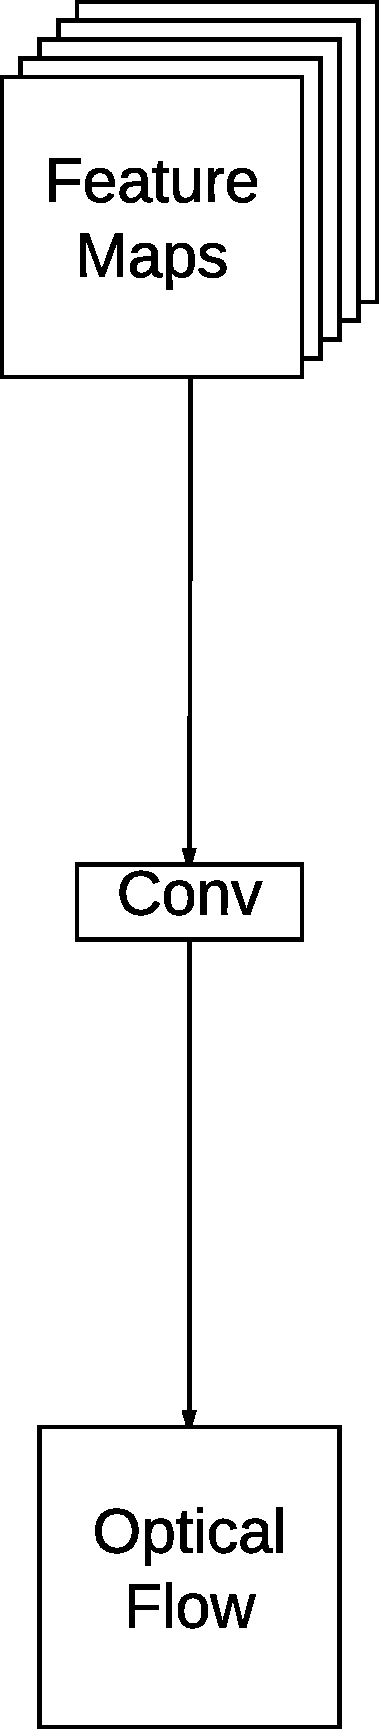
\includegraphics{Pic/PDF/NetworkStructure/Normal.pdf}}}
  &
  \resizebox{0.21\textwidth}{!}{\rotatebox{0}{
  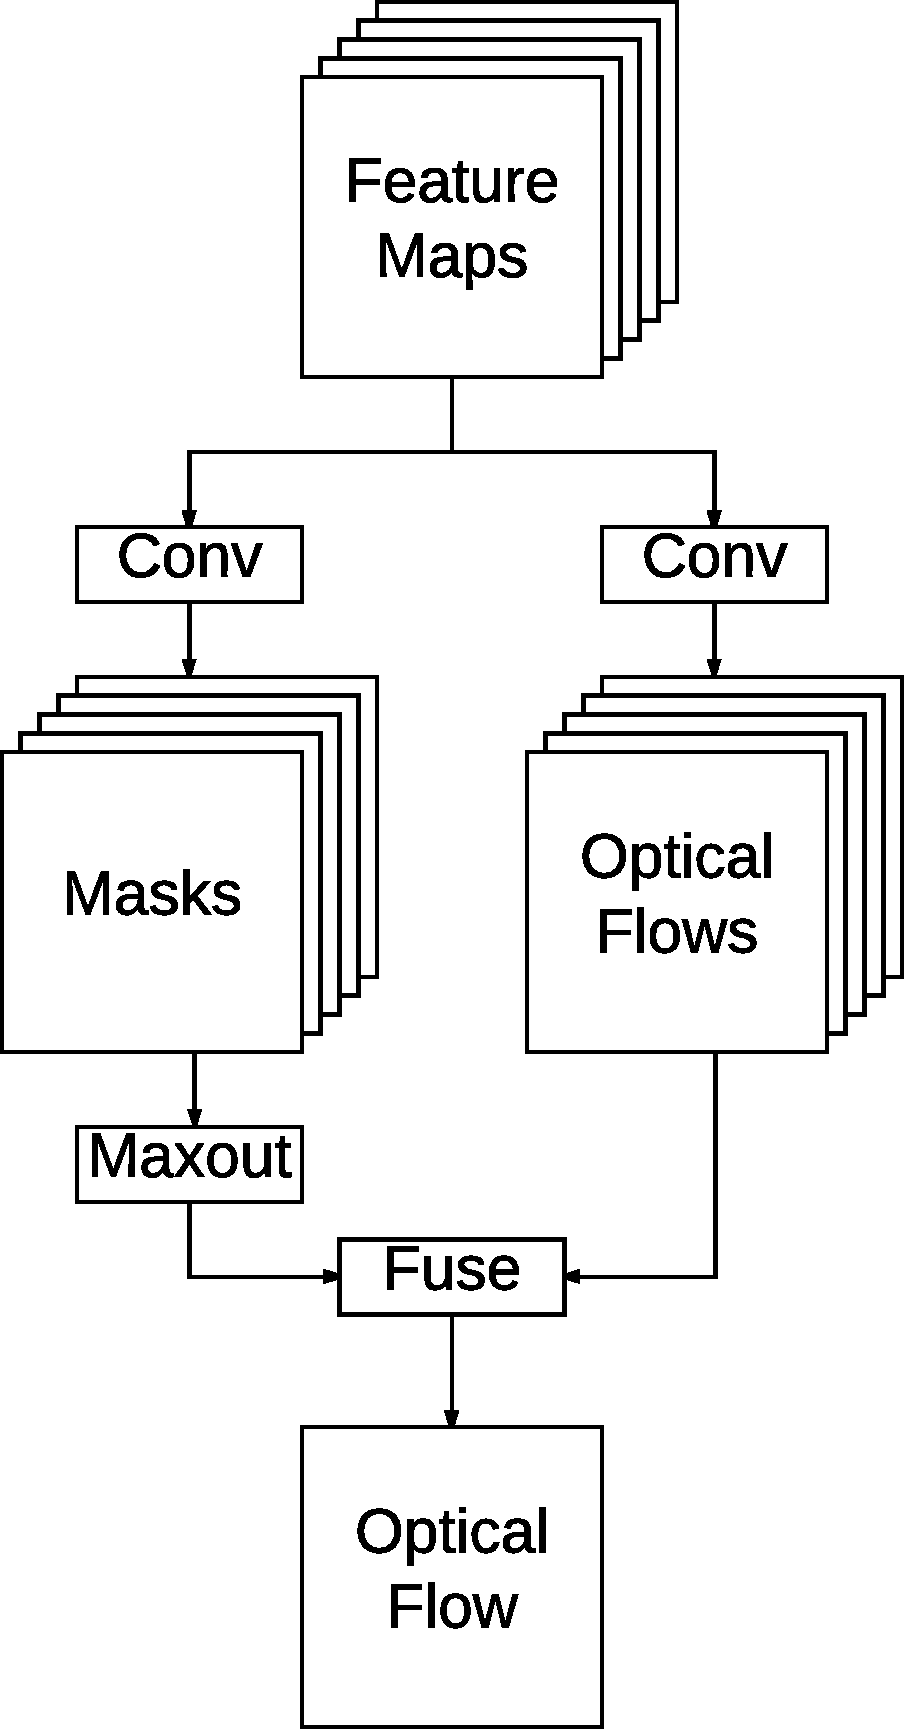
\includegraphics{Pic/PDF/NetworkStructure/MaskModule.pdf}}}
  \\
  a. Normal output & b. Soft-masks module 
  \\
\end{tabular}}
\caption{An illustration of the structure of the proposed soft-masks module compared with normal linear optical flow output.}
\label{fig: soft-masks module}
\end{figure} 

\subsection{Soft-masks module}
FlowNet~\cite{7410673} is the first work that uses deep convolutional neural network for flow estimation. The network architecture used by FlowNet is very similar to classical structure of auto-encoder, where optical flows are generated using deconvolution at each scale level of the image pyramid. To refine estimation of the flows, shortcuts are built to connect layers of corresponding level in encoder and decoder. Let's take a look at a single computation of convolution, and for simplicity, let's assume $f$ represents both horizontal and vertical components of an output flow. Given $X \in \mathbb{R}^{s\times s \times c}$, representing a volume feature vector in the input feature volume, inputted to output layer,  where $s$ is kernel size and $c$ is number of channels. FlowNet employs a linear activation to compute optical flow:

\begin{equation}
f = X^T W + b
\end{equation}

\begin{figure}[h]
\centerline{
\begin{tabular}{c}
  \resizebox{0.3\textwidth}{!}{\rotatebox{0}{
  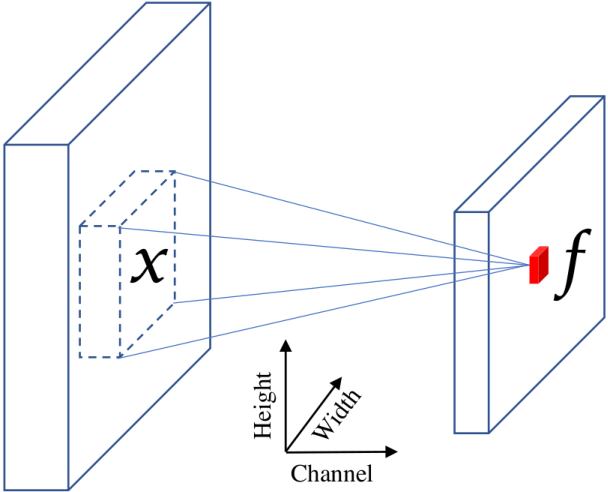
\includegraphics{Pic/PDF/conv_demo-crop.pdf}}}
  \\
\end{tabular}}
\caption{An illustration of annotation used in convolution.}
\label{fig: conv_layer}
\end{figure} 

Given actual optical flow field a nonlinear and piece-wise smooth representation of motions contained in images, using linear function to fit the flow field is less accurate. We introduce a soft-masks module in this paper. The proposed module can be used to replace the linear output of optical flow estimation. We will show that by using this module, we are able to separate optical flow field to multiple layers. Flow estimation in each layer is smooth and can be estimated using a quadratic function, which results in a more accurate and flexible optical flow estimation. 

An illustration of soft-masks module is shown in Figure~\ref{fig: soft-masks module}. The essential part of the soft-masks module is its dual-branch structure which contains mask branch and optical flow branch. The same input feature maps represented as a set of volume feature vectors, $X \in \mathbb{R}^{s\times s \times c}$ thus are imported to both branches. The most significant contribution of this work is to separate one optical flow field to multiple layers. For a separation of $k$ layers. $k$ masks will be generated in mask branch as illustrated in Figure~\ref{fig: soft-masks module}, which requires $k$ convolutional filters labeled as $\{W_n^m, b_n^m\}_{n=1}^k$ being used in mask branch. Correspondingly, the same number of filters are used in optical flow branch which are labeled as $\{W_n^f, b_n^f\}_{n=1}^k$. Then the mask and intermediate optical flow could be computed as following:

\begin{align}
\label{eqn: computation of masks and flows}
m_n =& X^T W_n^m + b_n^m &\! \text{for $n = 1\dots k$} \nonumber\\
f_n =& X^T W_n^f + b_n^f &\! \text{for $n = 1\dots k$}
\end{align}
Thus, give $k$ filters used in both branches, we will obtain $k$ corresponding pairs of mask and intermediate optical flow. Basically, by using $k$ filters in optical flow branch and generating $k$ intermediate optical flow, we assume each filter will work independently and being active only to a single type or a few types of object motions. Correspondingly, filters in mask branch are expected to have some behaviors that each of the generated masks which indeed are active maps should be high active for certain types of motions in some region and low active for other types of motions in other regions. This inspires us to use a maxout operation to extract mask entries with maximal activation along channel axis. So, after maxout operation, for each mask $m_n, n=1\dots k$, all entries will be zero-out except entries whose activation value are maximal in the some region among all masks. We denote masks after maxout as $\{m_n'\}_{n=1}^k$. Thus, there is no intersection among masks in $\{m_n'\}_{n=1}^k$ and the union of all $m_n', n=1\dots k$ has activation in full region. The maxout can be represented as following:

\begin{equation}
\label{eqn: maxout}
m_n'=
\begin{cases}
m_n, & \text{if}\ m_n = \max\limits_{p=1\dots k}(m_p) \\
0, & \text{otherwise}
\end{cases} \quad \text{for $n = 1\dots k$}
\end{equation}

It could be seen from Equation~\ref{eqn: maxout}, the masks after maxout are not converted to binary masks. This is the reason why the module is called soft-masks module. 

\begin{figure}[h]
\centerline{
\begin{tabular}{c}
  \resizebox{0.3\textwidth}{!}{\rotatebox{0}{
  
\includegraphics{Pic/PDF/PicHere.pdf}}}
  \\
\end{tabular}}
\caption{An illustration of how maxout is working for soft-masks module.}
\label{fig: maxout demo}
\end{figure} 

Masks after maxout operation are applied to corresponding intermediate optical flows by element-wise multiplication which is shown in below:

\begin{figure}[th]
\centerline{
\begin{tabular}{c}
  \resizebox{0.48\textwidth}{!}{\rotatebox{0}{
  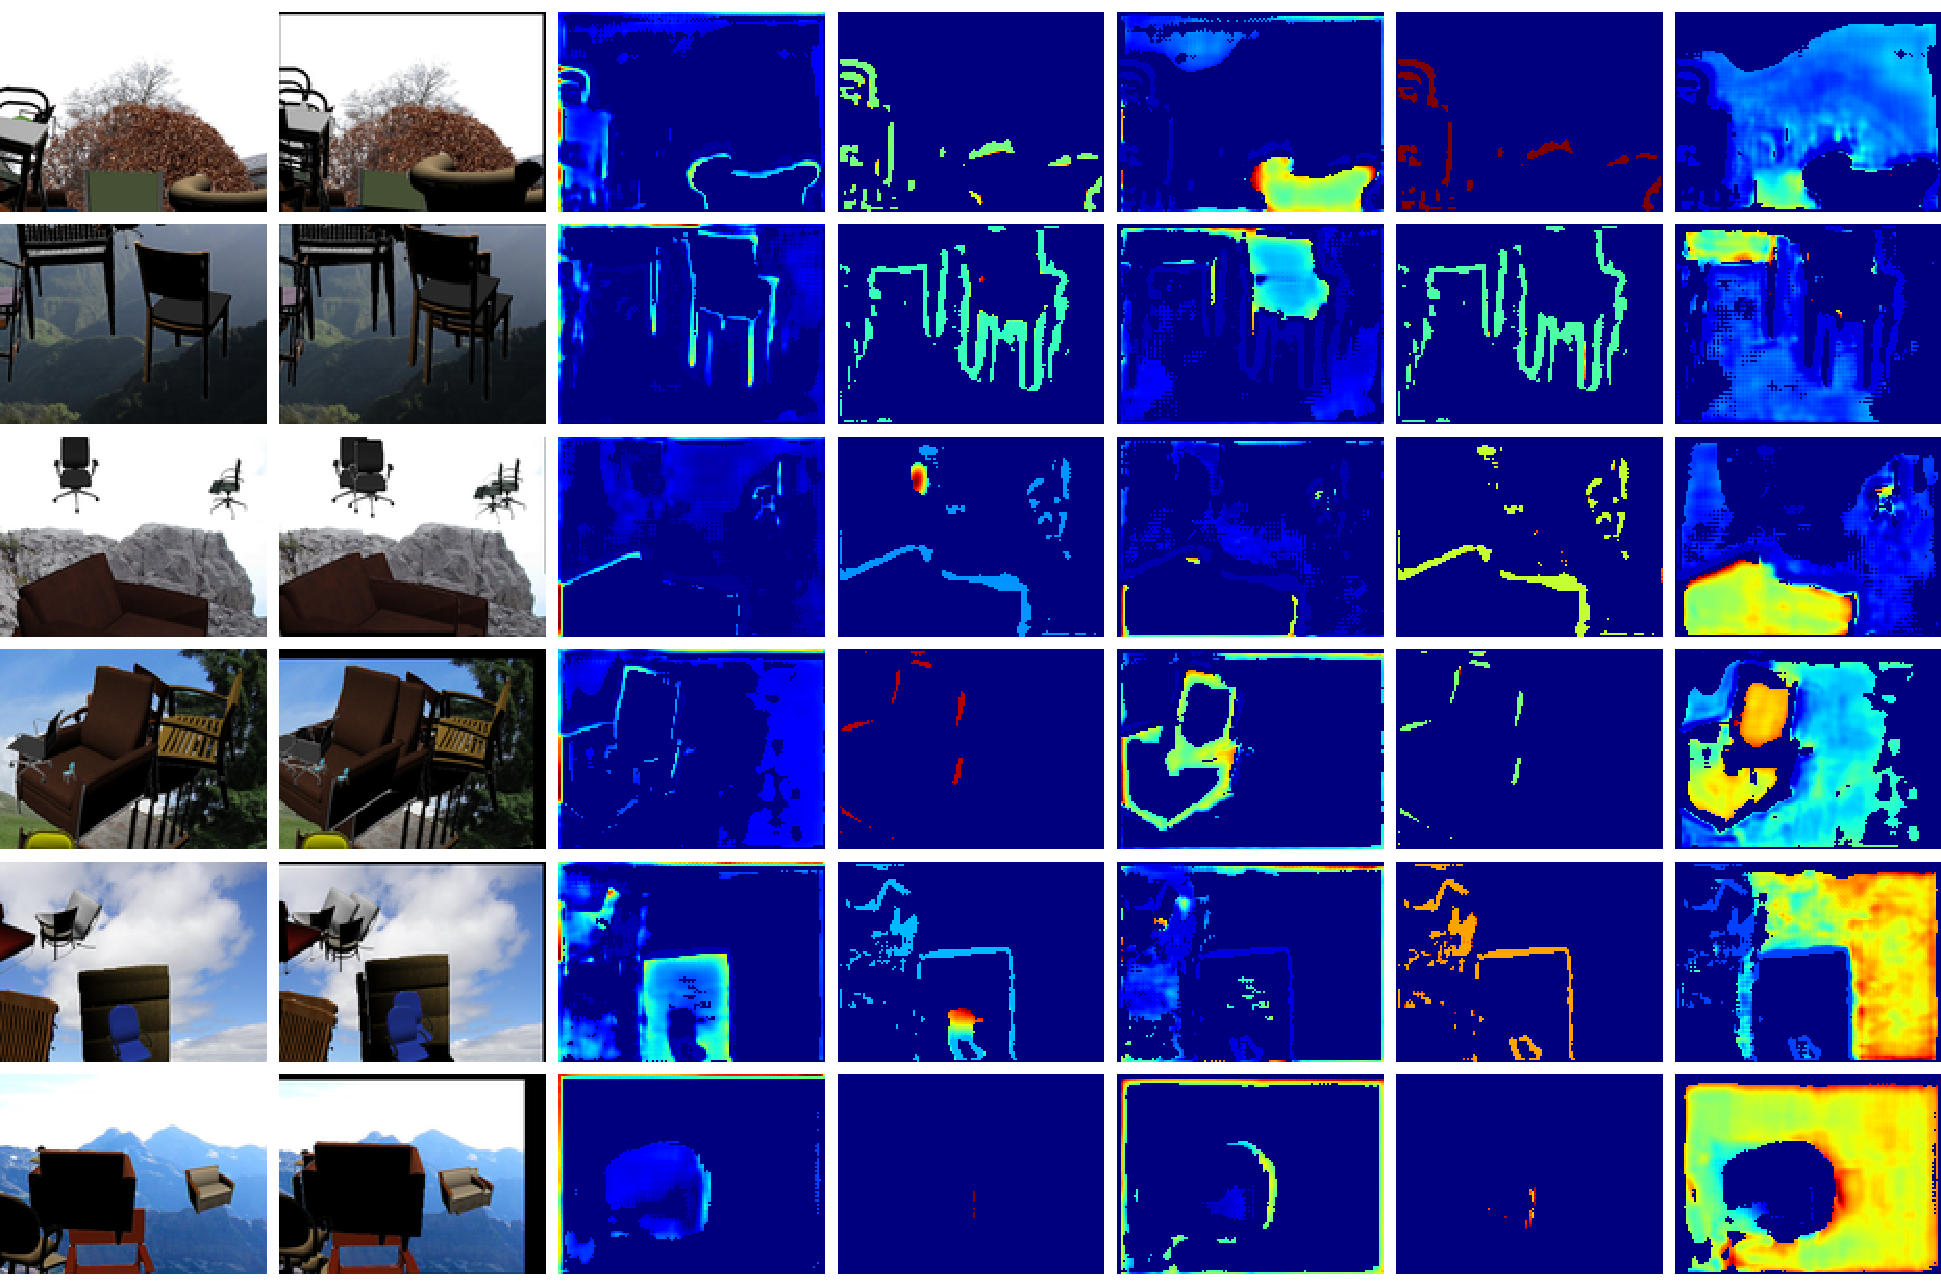
\includegraphics{Pic/PDF/Masks.pdf}}}
  \\
\end{tabular}}
\caption{Examples of generated masks using the proposed soft-mask module. In this example, five masks are generated for each input image pair.Mask values are rearranged to ones between 0 and 1 for rendering.}
\label{fig: maxout demo}
\end{figure} 

\begin{equation}
\label{eqn: maxout}
f_n'=
\begin{cases}
m_n' \times f_n, & \text{if}\ m_n' \neq 0 \\
0, & \text{otherwise}
\end{cases} \quad \text{for $n = 1\dots k$}
\end{equation}
Results of the above computation is a set of disjoint optical flow layers, each of which represent a certain type of motion. An illustration of how soft-masks module works is show in Figure~\ref{fig: maxout demo} and results of generated masks are show in Figure~\



\subsection{Quadratic fitting of optical flows}
Objects move in different ways in images, which results in different types of motion. The underlying optical flows thus are non-linear and locally piece-wise smooth. 

There are two consequences of using soft-masks module that could make estimation of the optical flow easier. The first advantage of using soft-masks module originate from usage of maxout in generating masks. By keeping only the maximal value among all masks, the optical flows are forced to be separated to multiple disjoint layers. Theoretically proofing maxout will result in a precise cut along motion boundary is challenging and is still under our investigation. However, qualitative results shown in Figure~\ref{fig: maxout demo} demonstrate that soft-masks module enable resulting masks to separate flow field to pieces according to detected motion types. In addition, the masks detects boundary of each piece as well, which enables estimation of optical flows on boundary more accurate.  Secondly, The estimation of optical flows using the proposed soft-masks module is quadratic in terms of feature maps $X$ inputed to the module.

To show this, given the computation of masks and intermediate optical flows shown in Equation~\ref{eqn: computation of masks and flows}, the computation of non-zero $f_n'$ could be written as:

\begin{align}
f_n' & = m_n' \times f_n \nonumber\\
	 & = (X^T W_n^m + b_n^m) \times (X^T W_n^f + b_n^f) \nonumber\\
	 & = W_n^m X X^T W_n^f + X^T(b_n^f W_n^m + b_n^m W_n^f) + b_n^m b_n^f
\end{align}
As shown in above equation, the representation of $f_n'$ is quadratic in terms of variable $X$.

To better illustrate the difference of using soft-masks module with respect to linear output, a 1D example is show in Figure~\ref{fig: quadratic demo}. In the example, function values are smooth in three separate ranges. The improvement of fitting data using piecewise quadratic function over linear function could be seen from this example. 

\begin{figure}[h]
\centerline{
\begin{tabular}{ccc}
  \resizebox{0.15\textwidth}{!}{\rotatebox{0}{
  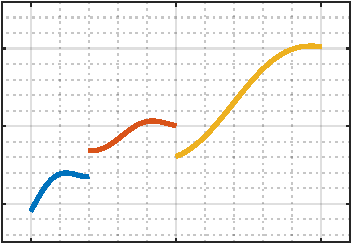
\includegraphics{Pic/PDF/QuadraticFuncDemo/FitDemo_1-crop.pdf}}}
  &
  \resizebox{0.15\textwidth}{!}{\rotatebox{0}{
  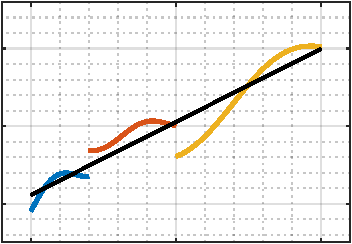
\includegraphics{Pic/PDF/QuadraticFuncDemo/FitDemo_2-crop.pdf}}}
  &
  \resizebox{0.15\textwidth}{!}{\rotatebox{0}{
  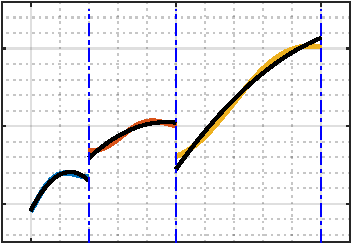
\includegraphics{Pic/PDF/QuadraticFuncDemo/FitDemo_3-crop.pdf}}}
  \\
  A & B & C
  \\
\end{tabular}}
\caption{A: Given data. B: Fitting using linear function. C: Fitting using piece-wise quadratic function.}
\label{fig: quadratic demo}
\end{figure} 

\subsection{Regularization for Unsupervised Training}
Training an unsupervised neural network for optical flow estimation is available by using network similar to FlowNet as a base optical flow inferring network followed by a spatial transform network (STN)~\cite{jaderberg2015spatial}. Existing works such as: DSTFlow~\cite{ren2017unsupervised}, USCNN~\cite{ahmadi2016unsupervised}, and back-to-basic unsupervised FlowNet (bb-FlowNet)~\cite{DBLP:journals/corr/YuHD16} all follow the same framework and train  their train neural networks unsupervisely to minimize an objective defined in Equation~\ref{eqn: flow objective}.  To show the proposed soft-masks module can improve flow estimation under the same framework, we add the soft-masks module to FlowNet and use it as a base optical flow inferring network in unsupervised training framework.

Smoothness restriction which is used by all above mentioned unsupervised approaches plays a significant role in regularizing the local consistancy of optical flows.  We follow the traditional regularization term used to constraint deformation field~\cite{rohlfing2003volume}\cite{ashburner1999nonlinear} and define the regularization term used in Equation~\ref{eqn: flow objective} as following:

\begin{align*}
\varphi(\bold(u)_{\xi}, \bold(v)_{\xi}) = & \sum ((\frac{\partial^2\bold{u}}{\partial \bold{x}^2})^2+(\frac{\partial^2\bold{u}}{\partial \bold{y}^2})^2+2(\frac{\partial^2\bold{u}}{\partial \bold{x} \partial \bold{y}})^2) + \\ 
& \sum ((\frac{\partial^2\bold{v}}{\partial \bold{x}^2})^2+(\frac{\partial^2\bold{v}}{\partial \bold{y}^2})^2+2(\frac{\partial^2\bold{v}}{\partial \bold{x} \partial \bold{y}})^2)
\end{align*}


\section{Empirical Evaluation}
\label{sec: evaluation}
\subsection{Benchmark}
We evaluate our performance on three standard optical flow benchmarks: Flying Chairs~\cite{7410673},  Sintel~\cite{Butler:ECCV:2012}, and KITTI~\cite{geiger2012we}. We compare the performance of the proposed approach to both supervised methods such as: FlowNet(S/C)~\cite{7410673}, FlowNet 2.0~\cite{Ilg_2017_CVPR}, SPyNet~\cite{Ranjan_2017_CVPR} and DeepFlow~\cite{weinzaepfel2013deepflow}, EpicFlow~\cite{revaud2015epicflow} and unsupervised methods including: DSTFlow~\cite{ren2017unsupervised}, USCNN~\cite{ahmadi2016unsupervised}, and back-to-basic unsupervised FlowNet (bb-FlowNet)~\cite{DBLP:journals/corr/YuHD16}. 

\subsection{Proposed Network Structure}
The goal of this paper is not to show a brand new design of a network and superior performance could be obtained using the network, instead, we are going to show performance improvement could be obtained by replacing normal optical flow output layer with soft-masks module. Based on this intention, we choose FlowNetS and FlowNetC as our base networks and replace their optical flow output layers with soft-masks module. Since we highlight the layered flow estimation (LOFE) in this paper, we term the resulting networks modified from FlowNet as FlowNetS+LOFE and FlowNetC+LOFE. 

One thing worth noticing is that although we chosen FlowNet to work on in our work, but since soft-masks module basically works as an add-on to a network, it can be used on wider selections of networks and vision tasks such as image segmentation~\cite{long2015fully}\cite{noh2015learning}, depth estimation in range images~\cite{eigen2014depth}\cite{eigen2015predicting}, etc..

\subsection{Evaluation of Soft-masks Module}
Since we replaced simple linear output layer in FlowNet(S/C) with a relatively more complicated soft-masks module, one obvious question about our result is whether we obtained them by using a model with more coefficients rather than by the way of how soft-masks module works. Therefore, to better investigate the mechanism of soft-masks module, we compared the FlowNetC+LOFE with another two networks in which we slightly changed the structures of the soft-masks module.

In the first network, given the proposed structure as FlowNetC+LOFE, we removed maxout operation from soft-masks module and keep all other configuration the same. We term the resulting network as FlowNetC+LOFE-v1. In this case FlowNetC+LOFE-v1 will have the exact same number of coefficients as FlowNetC+LOFE. For the second network, we further totally removed the mask branch from soft-masks module and leave the intermediate optical flow branch only. The second network is denoted as FlowNetC+LOFE-v2.  


\subsection{Training Details}

\subsection{Results}

\section{Discussion and Summary}

{\small
\bibliographystyle{ieee}
\bibliography{mybib}
}

\end{document}
